\part{Implementierung der Turing-Welchman-Bombe}\label{ch:impl_bombe}
%\section{Enigma-Maschine}\label{sec:impl_enigma}
%Um die Bombe in Software Nachzubilden, muss zuerst eine Enigma-Maschine nachgebildet werden.
%\subsection{Rotoren}\label{subsec:impl_enigma_rotor}
%Die Verdrahtung der Rotoren wurden als Vektor realisiert.
%Der zu permutierende Buchstabe wird hierfür als Index in den Vektor genutzt.


\chapter{Menü Algorithmus}\label{sec:cycle-finding-algorithm}
Um eine Turing-Welchman-Bombe in der Programmiersprache C nachzubilden, muss zuerst ein Algorithmus entworfen werden, welcher das Menü durch ein von dem Nutzer vorgegebenes Crib und 
%TODO
Geheimtext bildet.

Hierfür werden die einzelnen Buchstaben als Knoten mithilfe einer Struktur dargestellt, welche zum einen den Buchstaben und zum anderen einen Vektor mit den anliegenden Auslegern beinhaltet.
Die Buchstaben-Tupel wurden ebenfalls als Struktur dargestellt, welche zwei Knoten, die Position im Crib und einen Booleschen Wert beinhaltet, welcher aussagt, ob dieses Tupel zum Zyklus beiträgt.

\begin{mylisting}
	\inputminted{C}{Implementierung/menu_structs.c}
	\caption{Realisierung der Menü Strukturen}
	\label{lst:code_impl_menu}
\end{mylisting}

%\begin{figure}
%\lstinputlisting[style=mystyle, caption={Realisierung der Menü Strukturen}, label={lst:code_impl_menu}]{Implementierung/menu_structs.c}	
%\end{figure}

Die Tupel werden nun in einer \glqq Nachschlagetabelle\grqq{} abgelegt.
Diese Tabelle hat 26 Stellen, repräsentativ für das Alphabet.
Ein jeweiliges Tupel wird sowohl unter dem ersten als auch unter dem zweiten Buchstaben abgelegt. 
Tupel wie \texttt{W:S} werden also unter \texttt{W} und unter \texttt{S} abgelegt.
Ein Tiefensuche-Algorithmus, der modifiziert wurde, um weniger \glqq gierig\grqq{} zu agieren, schlägt die Tupel in der Tabelle nach und markiert die besuchten Tupel.
%Bei dem Rücksetzverfahren der Tiefensuche wird die Markierung der Tupel, die nicht zum Zyklus beitragen entfernt.
Das Ergebnis ist eine gemessene, lineare Laufzeit.
\begin{marginfigure}
	\centering
	%	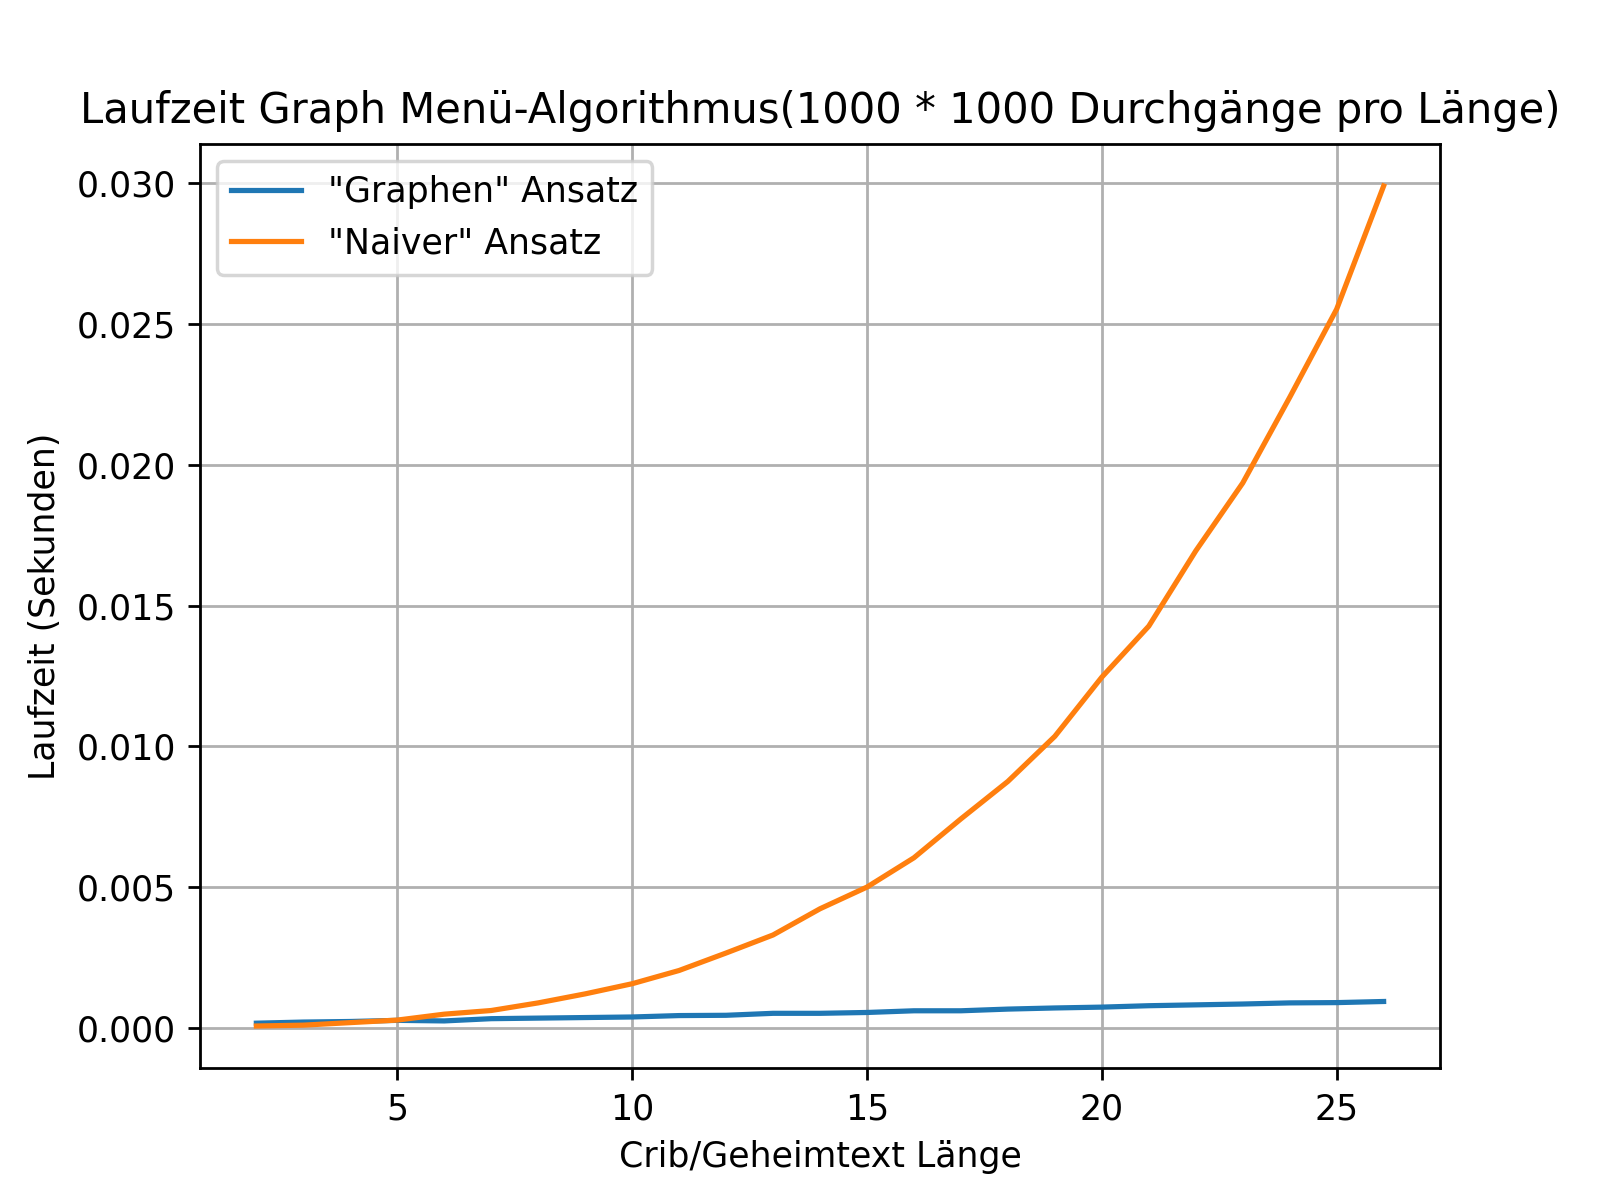
\includegraphics[width=.7\linewidth]{Turing Bomb/Crib-Cipher Loop/Runtime Graph Graph vs Force}
	\begin{tikzpicture}[scale=0.8]
		\begin{axis}[
			grid=major,
			xlabel={Inputvektor Länge},
			ylabel={Laufzeit (Sekunden)},
			axis lines=left,
			enlarge x limits={true},
			enlarge y limits={true},
			legend style={
				at={(0.4,1)},
				anchor=north,
				font=\small
			}
			]
			\addplot[thick, mark=none, gold] table[y=y1, x expr=\coordindex] {Turing Bomb/Crib-Cipher Loop/data.dat};
			\addlegendentry{"Graphen"-Algorithmus}
			\addplot[thick, mark=none] table[y=y2, x expr=\coordindex] {Turing Bomb/Crib-Cipher Loop/data.dat};
			\addlegendentry{"Naiver"-Algorithmus}
		\end{axis}	
	\end{tikzpicture}
	\caption{Der Laufzeit-Graph Menü-Algorithmus, getestet mit 1000 zufälligen Texten à 1000 Durchgänge.}
\end{marginfigure}
%\footnote{Es wurden Crib-Längen bis 26 betrachtet, um zu garantieren, dass die lineare Laufzeit bei einer maximalen Länge von 13 Buchstaben gegeben ist.
%Der Laufzeit-Graph ist im Anhang enthalten:~\cref{fig:app_menu_runtime}.}

Das Menü wird als Vektor von \texttt{CribCipherTuple} in einer Struktur mit der Länge abgelegt.
Da es erforderlich ist, eine eindeutige \glqq Route\grqq{} durch das Menü anzugeben, werden Tupel-Kombinationen bei den betroffenen Knoten als Ausleger angegeben. 
Die Bombe kann somit im Falle der \glqq Scramblersatz-Knappheit\grqq{} entscheiden, ob sie diesen (nicht notwendigen) Bestandteil des Menüs aufnehmen möchte.

\chapter{Modellierung der Turing-Welchman-Bombe}\label{sec:model}
\section{Scrambler}\label{subsec:impl_scrambler}
Wie in~\cref{subsec:vorbereitungen} erklärt, vernachlässigt die Bombe den Übertragzeitpunkt der Walzen.
Die Software-Implementation berücksichtigt ebenfalls die Übertragskerbe der Rotoren nicht.
%TODO Enigma Software gegeben erwähnen?
Die Verdrahtung der Scrambler wird als Vektor abgebildet, welcher wie in~\cref{fig:rot1_wiring} die Permutation für jeden Buchstaben speichert.
Die Buchstaben werden jedoch nicht in der typischen ASCII-Kodierung gespeichert, sondern auf den Wertebereich 0--25 abgebildet.
%TODO check
Mit dem Resultat kann somit direkt der Vektor des nächsten Scramblers indiziert werden.
Es muss zudem die Walzenlage mitgeführt werden, welche mit dem zu permutierenden Buchstaben addiert wird, um den Vektor-Index zu bilden.
Der Wertebereich wird durch eine Modulo-Operation zwischen 0 und 25 gehalten.

\section{Terminal}\label{subsec:impl_terminal}
Die Kontakte der Terminals werden als Struktur dargestellt.
Es beinhaltet einen 32-Bit-Integer, welcher als Bitvektor mit 26 seiner Stellen die aktiven Kontakte repräsentiert.
Die Anzahl der aktiven Kontakte wird ebenfalls als Integer mitgeführt.
Da es in Bezug auf die Laufzeit medioker ist, alle 26 Stellen des Bitvektors traversieren zu müssen, um zu überprüfen, welche der 26 Kontakte aktiv sind, wurde ein normaler Vektor eingeführt, der die aktiven Kontakte \glqq dicht\grqq{} speichert.
%TODO Artikel vor Nummer
Zuletzt wird der Buchstabe/die Nummer des jeweiligen Kontakts in der Struktur gespeichert.

\begin{mylisting}
	\inputminted{C}{Implementierung/terminal.c}
	\caption{Realisierung der Terminals}
	\label{lst:code_impl_terminal}
\end{mylisting}

Permutiert ein Scrambler einen Buchstaben, wird mithilfe des Bitvektors überprüft, ob dieser Kontakt bereits aktiv ist.

Hierbei gibt es zwei Szenarien:
\begin{enumerate}
	\item Der Kontakt ist inaktiv: In dem Bitvektor wird die repräsentative Stelle aktiviert, der Buchstabe wird in dem normalen Integer-Vektor abgelegt und die Anzahl der aktiven Verbindungen inkrementiert.
	
	\item Der Kontakt ist aktiv: Dieser Buchstabe wird ignoriert. 
\end{enumerate}

Die Terminal-Struktur beinhaltet einen Vektor mit 26 Kontakte und einen Zeiger auf den Kontakt des Test-Registers.
Bei dem Test-Register wird hierbei nicht von einem \glqq normalen\grqq{} Kontakt unterschieden.

\section{In und Outs}\label{subsec:impl_in_und_outs}
Die In- und Out-Kontakte werden mit dem dazugehörigen Scramblersätzen als Knoten dargestellt.
Sämtliche Verbindungen durch Kabel und Brücken-Konnektoren des analogen Originals werden hier durch Zeiger auf Kontakte ersetzt, so auch die In- und Out-Kontakte.

\section{Commons}\label{subsec:impl_commons}
Aufgrund der Einfachheit wurden die Commons in dieser Software-Imple\-men\-tation \glqq weg abstrahiert\grqq.
Diese wurden durch Zeiger auf den gleichen Kontakt ersetzt.
Die Anzahl der Kontakte pro Commons und die Gesamtzahl der verwendeten Commons wurde gezählt, sodass diese nicht die Anzahl des analogen Originals überschreiten.

\section{Diagonalbrett}\label{subsec:impl_diagonal_board}
Das Diagonalbrett als native Datenstruktur darzustellen, hat sich als ein eher schlechter Einfall herausgestellt.
Eine Möglichkeit, das Verhalten mit einer Datenstruktur zu imitieren, ist es, die einzelnen Kontakte der Terminals als Vektor mit Zeiger auf Booleschen Werten abzubilden.
Hierbei zeigt zum Beispiel der \emph{a}-Kontakt des \emph{B}-Terminals und der \emph{b}-Kontakt des \emph{A}-Terminals auf den gleichen Booleschen Wert.
Somit ist die Verbindung $A \Leftrightarrow B$ abgebildet.
Jedoch wäre es hier abermals nötig, den gesamten Vektor zu traversieren, um die aktiven Kontakte herauszufinden.
Die entsprechenden Kontakte müssten nun wieder einen normalen Vektor besitzen, in dem die aktiven Kontakte \glqq dicht\grqq{} stehen, damit die Scrambler effektiv arbeiten können.
Somit wäre es hier abermals notwendig, die Kontakte separat zu behandeln.

Aus diesem Grund wurde die Funktion des Diagonalbrettes in einer Funktion gekapselt:

\begin{mylisting}
	\inputminted{C}{Implementierung/diag_method.c}
	\caption{Realisierung des Diagonalbrettes}
	\label{code_impl_diag_board}
\end{mylisting}

%TODO TuringBombe Struct erklären?
Diese Funktion erhält drei Argumente: Einen Zeiger auf eine \texttt{TuringBombe} und zwei Integer, repräsentativ für die zwei Terminal-Buchstaben, die aktiviert werden sollen.

\chapter{Algorithmus der Implementation}\label{sec:algorithm_bombe}
Im Gegensatz zur \glqq echten\grqq{} Bombe, welche eine Steckerbrett-Hypothese für die jeweils 17576 Walzenstellungen einer Walzenlage testet, testet die Software-Nachbildung eine Hypothese für alle Walzenstellungen der 60 möglichen Walzenlagen.
Eine modifizierte Breitensuche traversiert die Knoten des aufgespannten Graphen der \glqq Scrambler-Knoten\grqq.
Da es aufgrund der Tupel-Kombinationen nicht genügt, einige Knoten nur einmal zu besuchen, und das Diagonalbrett es schwierig macht, die Datenstruktur der Knoten linear zu durchlaufen, wird erneut eine \glqq Nachschlagetabelle\grqq{} benötigt.
Die Nachschlagetabelle besitzt 26 Stellen, jeweils für die 26 Terminal-Kontakte.
Die Knoten, die durch den In-Kontakt mit einem jeweiligen Terminal verbunden sind, werden in dieser Tabelle abgelegt.
Zuerst werden alle Scrambler-Knoten, die durch den In-Kontakt mit dem Test-Register verbunden sind, in die Warteschlange eingereiht. 
Danach werden die Commons der jeweiligen Knoten eingereiht und als Letztes die Knoten, welche an jene Kontakte anliegen, die durch direkte Permutation der Scrambler oder durch das Diagonalbrett aktiviert wurden.
Wird durch die Permutation eines Scramblers in dem mit ihm verbundenen Out-Kontakt kein neuer Kontakt aktiv, so werden die Knoten, welche durch den In-Kontakt mit dem jeweiligen Kontakt verbunden sind, nicht eingereiht.
%wird dieser Knoten als \glqq besucht\grqq{} gekennzeichnet und nicht mehr in die Warteschlange eingereiht.
Ist die Warteschlange leer, ergo keine Permutationen mehr möglich, wird das Test-Register überprüft.
%sind alle Permutationen abgeschlossen und das Test-Register wird überprüft.
Ergeben die Permutationen keine gültige Konfiguration, werden alle Kontakte die durch Permutation oder Diagonalbrett aktiviert wurden, deaktiviert. 
%und Knoten als nicht besucht gekennzeichnet.
Die Software-Nachbildung hält nach den in~\cref{subsec:test-register} beschriebenen Regeln.
%In Pseudocode könnte man den Algorithmus der Bombe so darstellen:
%\begin{algorithm}[htbp]
%	\caption{Bombe Algorithmus}
%	\begin{algorithmic}
%			\Procedure{Bombe}{$p_0 \dots p_{n-1} :$ [Char], $c_0 \dots c_{n-1} :$ [Char]}
%			\ForAll{\textsl{rotors} $\in$ \textbf{permut(rotor order)}, \textsl{pos} $\in$ \textbf{[AAA $\dots$ ZZZ]}}
%			\State plugs: Char $\rightarrow \{ $Char$\}$
%			\State plugs$(p_0)\ \cup= \{\textbf{'A'}\}$
%			\While{\textsl{plugs} changing}
%			\ForAll{\textsl{i} $\in$ \textbf{[0\dots n--1]}}
%			\State plugs($c_i$) $\cup=$ $\bigcup_{p \in \text{plugs}(p_i)}$ encrypt(\textsl{rotors, p, pos}+\textsl{i})
%			\State plugs($p_i$) $\cup=$ $\bigcup_{p \in \text{plugs}(c_i)}$ encrypt(\textsl{rotors, p, pos}+\textsl{i})
%			\EndFor
%			\EndWhile
%			\If{$\forall$ \textsl{S} $\in$ \textbf{cod(plugs)}: \#S < \#Char}
%			\State report(\textsl{pos, plugs})
%			\EndIf
%			\EndFor
%			\EndProcedure
%		\end{algorithmic}
%	\label{alg:algorithm}
%\end{algorithm}
